\section{System}
\label{sec:system}
\begin{figure*}[t]
\centering
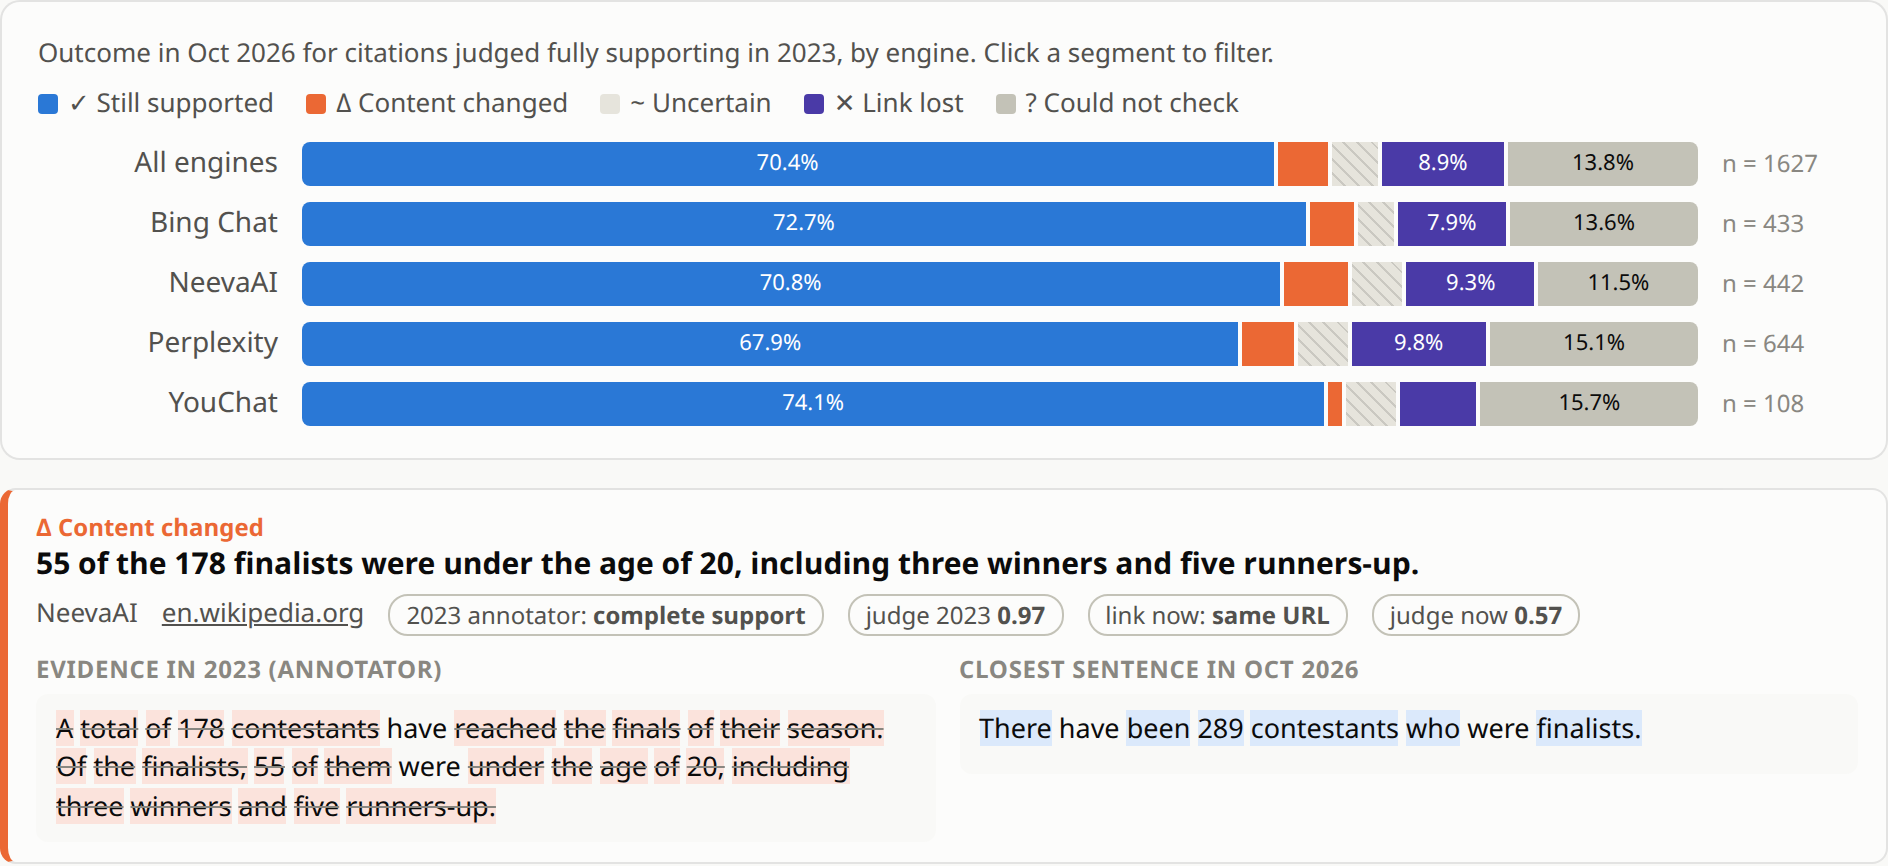
\includegraphics[width=0.77\textwidth]{figures/ui_explorer.png}
\caption{CiteDrift explorer. Top: outcome in October 2026 of all citations that annotators judged fully supporting in 2023, including those that could not be checked, per engine (segments filter the list). Bottom: one pair; the 2023 evidence and today's closest sentence are aligned word by word: the page is still online, some figures changed, and the judge's score dropped from \figPthen to \figPnow.}
\label{fig:ui}
\end{figure*}
CiteDrift takes an answer with citation markers (\texttt{[1]}, \texttt{[2]}, \dots), the list of cited URLs and, optionally, the date of the answer. It splits the answer into sentences, pairs every sentence with the citations it carries, and processes each statement--citation pair in four steps (Fig.~\ref{fig:ui}).

\textbf{1. Link state.} Each URL is requested once by an identified client with per-host spacing. A plain HTTP request is not enough to decide that a link is lost: in our measurement, \calBlockedReachable{} of the \calBlockedTried{} URLs that answered a plain request with 401/403/429 and were re-opened opened normally in an ordinary browser, and \calFiltered{} URLs were answered by our own network's web filter rather than by the site. CiteDrift therefore (i) recognises filter and bot-wall pages by their text, (ii) re-opens refused pages in an ordinary desktop browser (in the batch measurement for every refused page not answered by our network filter; on request in check mode); it does not solve challenges or bypass paywalls, and a page that appears only after a detected bot interstitial counts as a bot wall, and (iii) judges redirects by content, not by URL: a redirect counts as \emph{moved} if the new page still contains at least 30\% of the cited page's word 5-grams or keeps its title (thresholds set before the evaluation from pages that kept their URL and redirects to a site root; script in the repository), and as \emph{redirected elsewhere} otherwise; without a ``then'' page only redirects to a site root count as lost. With this rule \calRedirectMoved{} of \calRedirect{} redirects were moves. The resulting states fall into three groups: \emph{reachable} (same URL, moved), \emph{lost} (dead, error page, redirected elsewhere) and \emph{unverifiable} (bot wall, network filter, server or TLS error, time-out, empty page, not requested).

\textbf{2. Then and now text.} The ``now'' page is reduced to its main content with Trafilatura~\cite{Barbaresi_2021}; the full visible DOM text is judged as well and the higher score counts, so that an extraction miss is not mistaken for a content change. The ``then'' page is the Internet Archive capture closest to the answer date, or page text saved with a dataset when available (for Liu et al., text extracted by the dataset authors' HTML-to-text pipeline). Archive lookups that fail (e.g., HTTP~429) are reported as such and never read as ``the page did not exist''.

\textbf{3. Support judge.} MiniCheck-Flan-T5-Large~\cite{Tang_2024} (our re-implementation of its reference inference) scores the statement against every $\sim$500-word chunk of a page and keeps the best chunk. Because AI search answers often copy phrases from their sources, the MiniCheck logit is combined with the share of the statement's word 4-grams found on the page (logistic regression fitted on the development split). The decision threshold is fixed on the development split and used unchanged at both time points.

\textbf{4. Outcome.} A pair is \emph{not supported when cited} if the judge rejects the ``then'' page, \emph{link lost} or \emph{could not check} according to its link state, and \emph{still supported} if the judge accepts today's page. Because the judge errs, a rejection today alone is not called a change: a pair is \emph{content changed} only if, in addition, the passage that supported the statement then is no longer on today's page; if it is still there the pair stays still supported, and if the signals cannot be compared it is \emph{uncertain}. For flagged pairs, an optional explainer (Qwen2.5-7B-Instruct~\cite{qwen2025qwen25technicalreport}, 4-bit) reads the best passage and writes a one-sentence reason.

\textbf{Interface.} A single web application (FastAPI back end, plain HTML/JS front end) has two modes. The \emph{explorer} is a static page with our precomputed results on the Liu et al. data: per-engine outcome bars that act as filters, and one card per pair showing the statement, the annotator's 2023 evidence next to the closest sentence on today's page with a word-level diff, link state and both judge scores. The \emph{check} mode runs the full pipeline on a pasted answer on the user's own machine and streams each outcome as soon as its page has been fetched and judged; nothing the user submits leaves the machine except requests for the cited pages, their robots.txt files and their archive records.
